\documentclass{article}
\usepackage[utf8]{inputenc}
\usepackage{graphicx}
\usepackage{amsmath}
\usepackage{amsfonts}
\usepackage{float}
\usepackage{listings}
\usepackage{xcolor}
\usepackage[a4paper, margin=1in]{geometry}
\title{Homework 9}
\author{Steve Gillet}
\date{\today}

% Custom information
\newcommand{\className}{Course: Algorithmic Motion Planning – ASEN 5254-001 – Fall 2024}
\newcommand{\professorName}{Professor: Morteza Lahijanian}
\newcommand{\taName}{Teaching Assistant: Yusif Razzaq}

\begin{document}

% Title
\maketitle
\begin{center}
    \large{\className} \\
    \large{\professorName} \\
    \large{\taName}
\end{center}

\section*{Exercise 1.
Implement a GoalBiasRRT planner for systems with kinodynamical constraints of the form
\[
\dot{x}(t) = f(x(t), u(t)),
\]
where \( x(t) \in X \) is the state, and \( u(t) \in U \) is the control, and \( f : X \times U \rightarrow \mathbb{R}^n \) is the vector field. Assume that the workspace is a rectangle in \( \mathbb{R}^2 \) with \( x \in [x_{\min}, x_{\max}] \) and \( y = [y_{\min}, y_{\max}] \). The program should take a given problem
\[
P = (X, U, x_{\text{init}}, X_G, f),
\]
where
\begin{itemize}
    \item \( X \) is the state space,
    \item \( U \) is the control space,
    \item \( x_{\text{init}} \) is the initial state,
    \item \( X_G \subset X \) is the goal region, and
    \item \( f : X \times U \rightarrow \mathbb{R}^n \) is the vector field, defining the dynamics of the system,
\end{itemize}
and return a kinodynamically (i) feasible trajectory:
\[
\zeta = \left\{ (x_i, u_i, \Delta t_i) \in X \times U \times [0, 0.5] \mid 0 \leq i \leq T, \, x_0 = x_{\text{init}}, \, x_T \in X_G, \, x_{i+1} = x_i + \int_0^{\Delta t_i} f(x(t), u_i) \, dt \right\},
\]
(ii) trajectory length, (iii) time duration, and (iv) computation time. Note that duration \( \Delta t_i \in [0, 0.5] \).\\
Solve Workspace 1 from \textbf{Exercise 2 of Homework 2} using your kinodynamic RRT, considering the following (point) robots:
\begin{itemize}
    \item[(a)] \textbf{2-dimensional single integrator:}
    \[
    x = (x, y)^T
    \]
    \[
    \dot{x} = (u_1, u_2)^T
    \]
    \[
    x_{\text{init}} = (0, 0)^T
    \]
    \[
    X = [x_{\min}, x_{\max}] \times [y_{\min}, y_{\max}]
    \]
    \[
    U = [-1.5, 3] \times [-1.5, 3]
    \]
    \[
    X_G = \{x \in X \mid \|x_{\text{goal}} - x\|_2 \leq 0.5\}
    \]
    \item[(b)] \textbf{3-dimensional first-order unicycle with wheel radius of \( r = 0.25 \):}
    \[
    x = (x, y, \theta)^T
    \]
    \[
    \dot{x} = (u_0 r \cos(\theta), u_0 r \sin(\theta), u_\omega)^T
    \]
    \[
    x_{\text{init}} = (0, 0, 0)^T
    \]
    \[
    X = [x_{\min}, x_{\max}] \times [y_{\min}, y_{\max}] \times [-\pi, \pi]
    \]
    \[
    U = [-2, 4] \times [-1.5, 1.5]
    \]
    \[
    X_G = \{(x, y, \theta) \in X \mid |x - x_{\text{goal}}| \leq 0.5, |y - y_{\text{goal}}| \leq 0.5, \theta \in [-\pi, \pi]\}
    \]
    \item[(c)] \textbf{5-dimensional second-order unicycle:}
    \[
    x = (x, y, \theta, \sigma, \omega)^T
    \]
    \[
    \dot{x} = (\sigma \cos(\theta), \sigma \sin(\theta), \omega, u_1, u_2)^T
    \]
    \[
    x_{\text{init}} = (0, 0, 0, 0, 0)^T
    \]
    \[
    X = [x_{\min}, x_{\max}] \times [y_{\min}, y_{\max}] \times [-\pi, \pi] \times [-3, 4] \times [-1.5, 1.5]
    \]
    \[
    U = [-1, 1.5] \times [-0.75, 0.75]
    \]
    \[
    X_G = [x_{\text{goal}} \pm 0.5] \times [y_{\text{goal}} \pm 0.5] \times [-\pi, \pi] \times [-2, 3] \times [-1, 1]
    \]
\end{itemize}
}

\subsection*{For each agent defined above, perform the following steps for \(W_1\).
i. Plot the motion plan and record the path length.}

\begin{figure}[H]
    \centering
    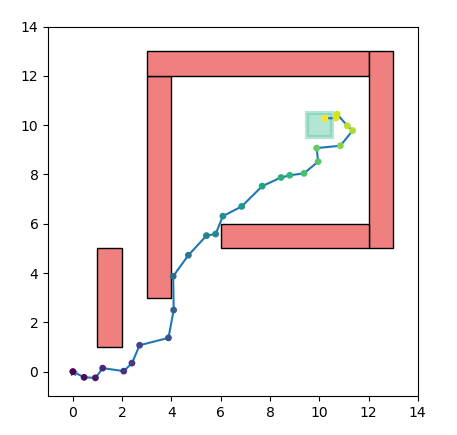
\includegraphics[width=0.7\textwidth]{1di0.png} 
    \caption{2D Single Integrator Workspace 1 Plot - Path Length: 19.0167.}
    \label{fig:1di0}
\end{figure}

\begin{figure}[H]
    \centering
    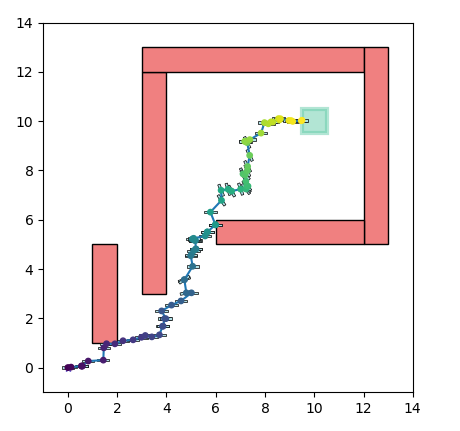
\includegraphics[width=0.7\textwidth]{1di2.png} 
    \caption{3D Second-Order Unicycle Workspace 1 Plot - Path Length: 18.6272.}
    \label{fig:1di2}
\end{figure}

\begin{figure}[H]
    \centering
    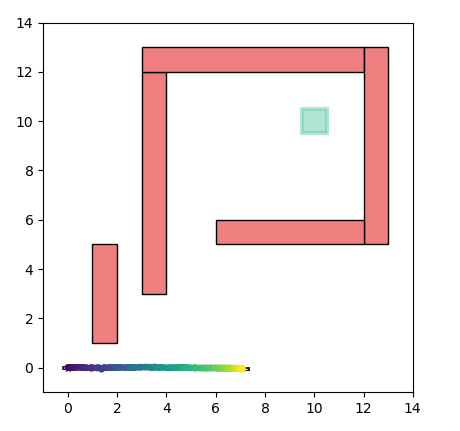
\includegraphics[width=0.7\textwidth]{1di4.png} 
    \caption{5D Second-Order Unicycle Workspace 1 Plot - Path Length: 7.27353.}
    \label{fig:1di4}
\end{figure}

\subsection*{(ii)
Vary \( n \) and number of \( u_{\text{samples}} \) (\( |u_{\text{samples}}| \)) and benchmark your solutions in three categories of number of valid solutions, path length, and computation time. For benchmarking, use 50 runs for each
\[
    (n, |u_{\text{samples}}|) \in \{ (50000, 1), (50000, 5), (50000, 10), (50000, 15) \}.
    \]    
    Show your results using boxplots.
}

\begin{figure}[H]
    \centering
    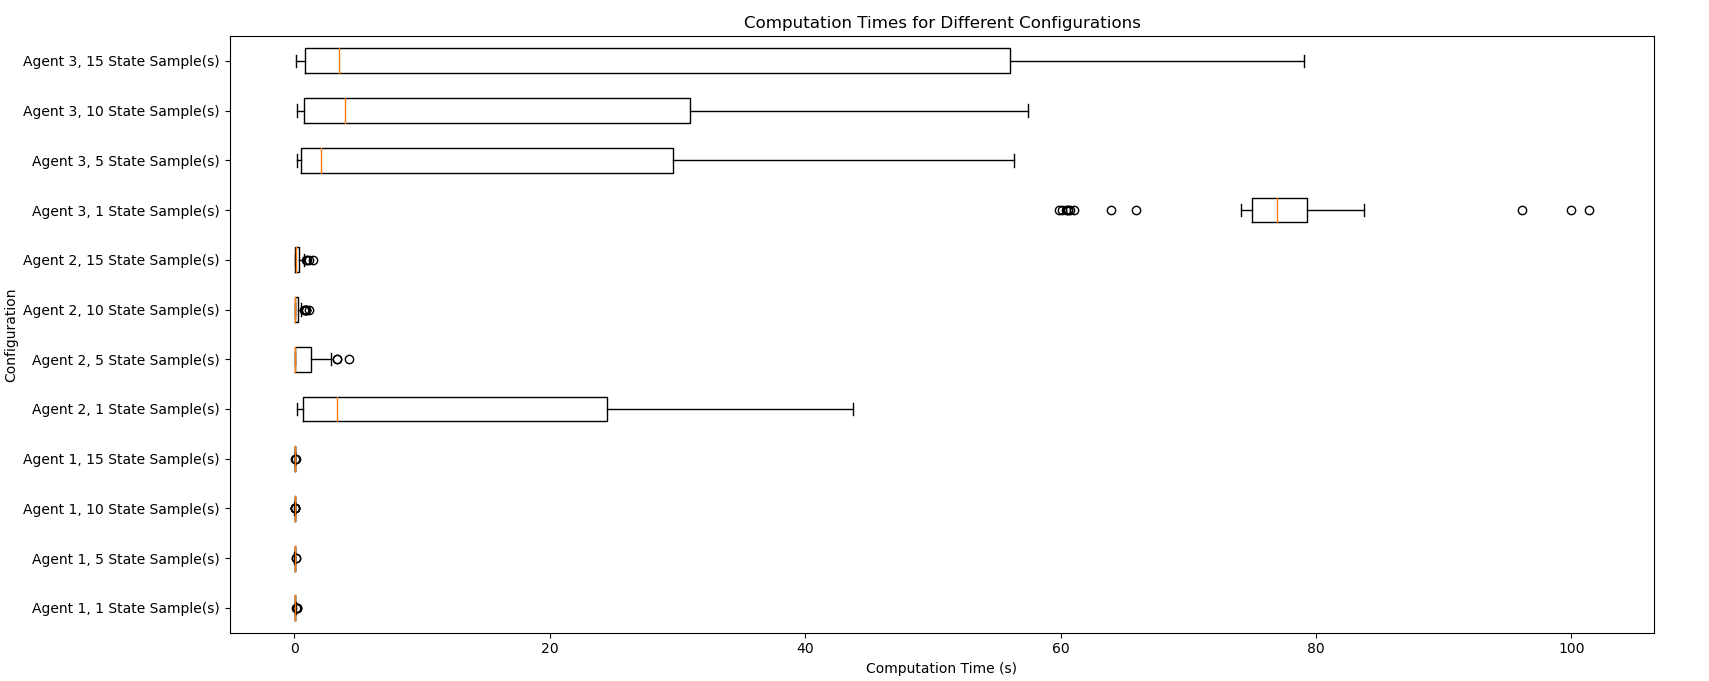
\includegraphics[width=0.7\textwidth]{1diiTimes.png} 
    \caption{Computation Times for the Various Agents with Various Control Sample Numbers}
    \label{fig:1diiTimes}
\end{figure}

\begin{figure}[H]
    \centering
    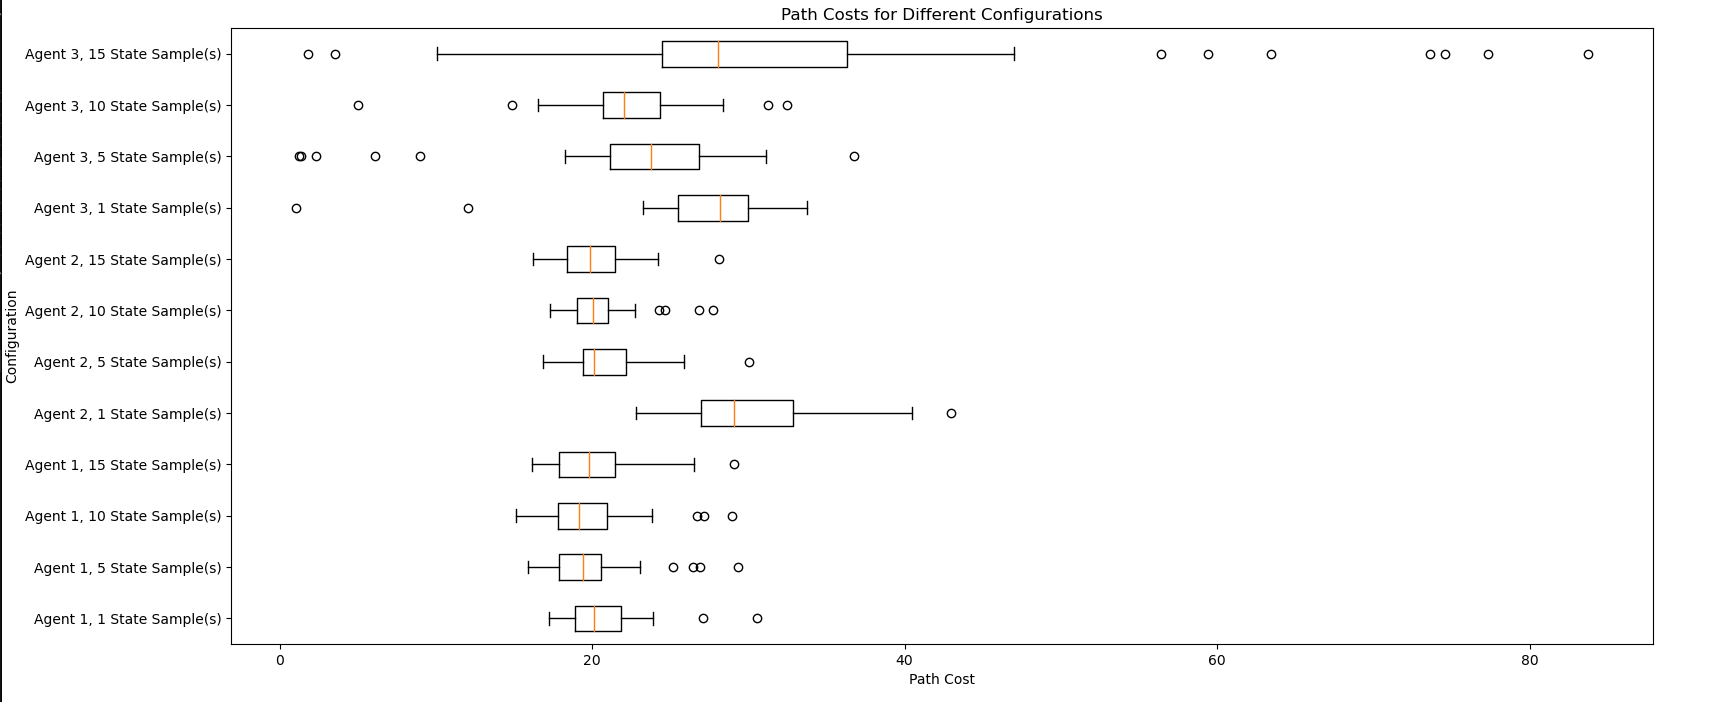
\includegraphics[width=0.7\textwidth]{1diiCosts.png} 
    \caption{Path Lengths for the Various Agents with Various Control Sample Numbers}
    \label{fig:1diiCosts}
\end{figure}

\begin{figure}[H]
    \centering
    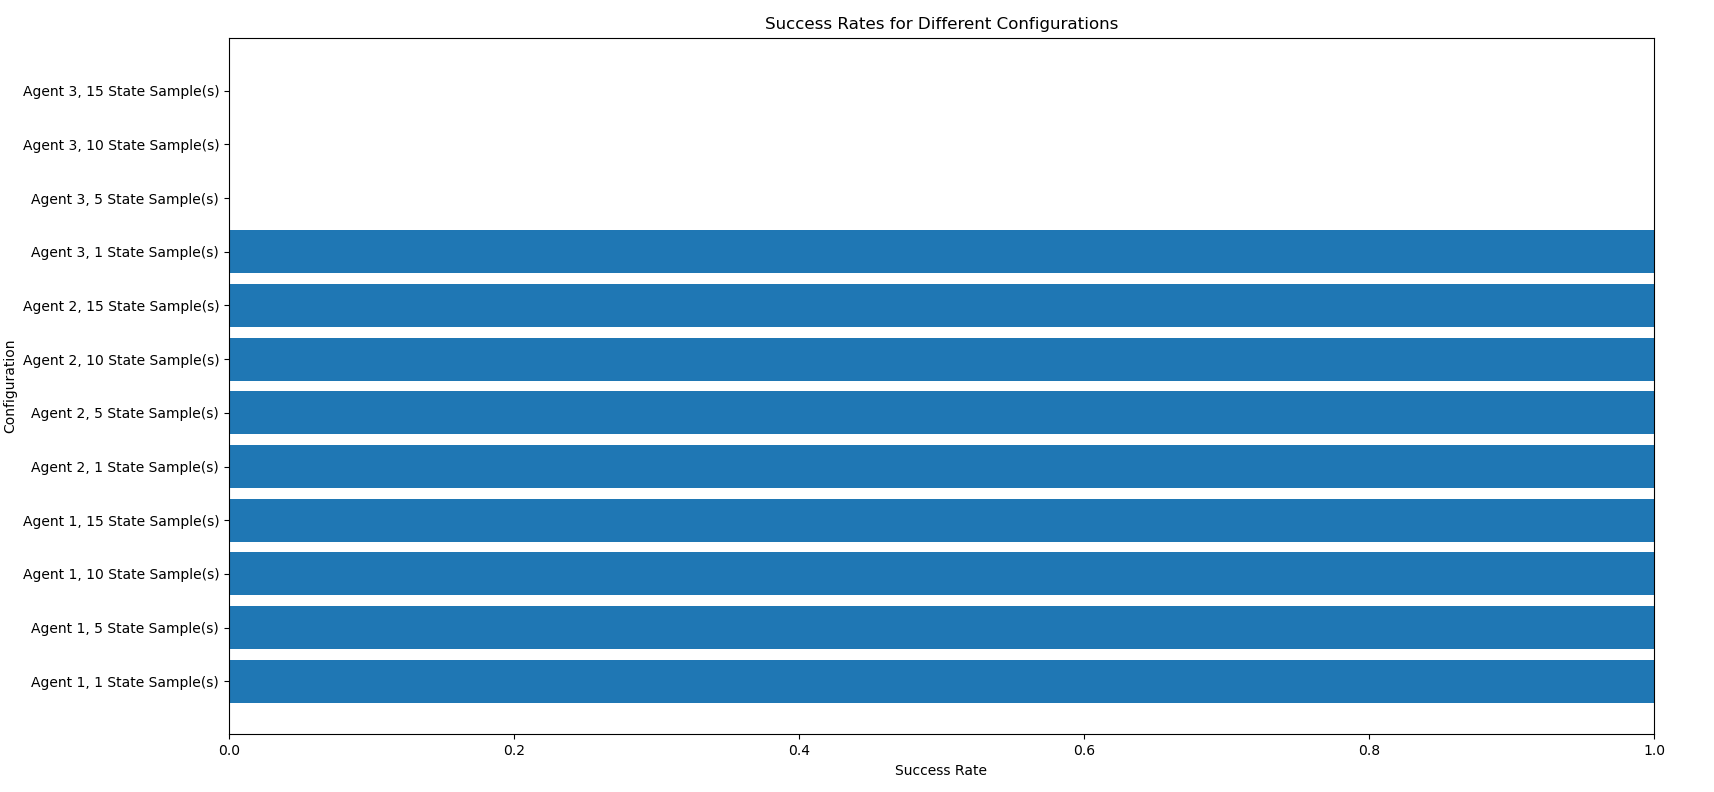
\includegraphics[width=0.7\textwidth]{1diiSuccesses.png} 
    \caption{Valid Paths for the Various Agents with Various Control Sample Numbers}
    \label{fig:1diiSuccesses}
\end{figure}


\subsection*{(iii)
Based on your empirical evaluations, what are the optimal values for \( n \) and \( u_{\text{samples}} \) in \( W_1 \)? Justify your answer.
}

15 control samples seems to be the way to go in my experience. The computation time is faster and then path cost is lower. The more the merrier.
I think very often what happens is the extra control samples allow the planner to find a better path sooner so it doesn't have to go through as many state samples to reach the goal.

\subsection*{(c) What distance metric did you choose and how was the distinction between dimensions for \(\mathbb{R}\) and \(\mathbb{S}\) handled?}

I chose to use the Euclidean distance metric, as it provides a straightforward and effective way of calculating the closest distance between two points. I did not make a distinction between dimensions in \(\mathbb{R}\) or \(\mathbb{S}\), since the Euclidean distance formula remains valid and applicable in any number of dimensions, making it suitable for both \(\mathbb{R}\)- and \(\mathbb{S}\)-dimensional spaces.

\subsection*{Exercise 2
Consider a robot modeled as a simple car that needs to perform a parallel parking maneuver in a two-dimensional workspace. The workspace, \( W \subset \mathbb{R}^2 \), includes a designated parking spot that the car must enter. The car has a rectangular shape with length \( L = 5 \) and width \( W = 2 \). Assume the distance between the front and rear axles is the same as \( L \). Note that the origin of the local frame of the car is located at the center of the rear axle (see the lecture notes).
The planning problem is defined as follows:
\[
x = (x, y, \theta, v, \phi)^T
\]
\[
\dot{x} = (v \cos \theta, v \sin \theta, \frac{v}{L} \tan(\phi), u_1, u_2)^T
\]
\[
x_{\text{init}} = (0.5, 5.5, 0.2, 0, 0)^T
\]
\[
X = [0, 22] \times [0, 8] \times [-\pi, \pi] \times [-3, 6] \times \left[-\frac{\pi}{3}, \frac{\pi}{3}\right]
\]
\[
U = [-1.5, 2] \times [-0.3, 0.3]^T
\]
\[
X_G = [7, 10] \times [1, 2] \times \left[-\frac{\pi}{30}, \frac{\pi}{30}\right] \times [-0.5, 0.5] \times \left[-\frac{\pi}{2}, \frac{\pi}{2}\right]
\]
with workspace obstacles:
\[
WO_1 : \begin{cases} v_1^1 = (0, 0), \\ v_2^1 = (15, 0), \\ v_3^1 = (7, 3), \\ v_4^1 = (0, 3) \end{cases}
\]
\[
WO_2 : \begin{cases} v_1^2 = (15, 0), \\ v_2^2 = (22, 0), \\ v_3^2 = (22, 3), \\ v_4^2 = (15, 3) \end{cases}
\]
}

\subsection*{(a) Plot the trajectory of the car as it maneuvers into the parking spot. Report the path length and computation time used to find the solution.}

\begin{figure}[H]
    \centering
    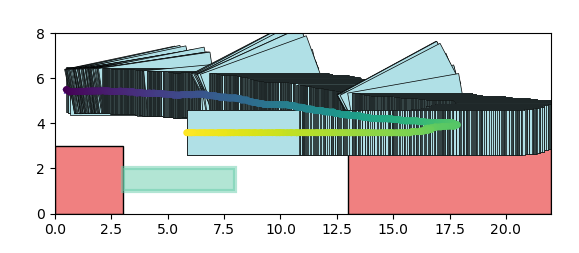
\includegraphics[width=0.7\textwidth]{2a.png} 
    \caption{Simple Car - Path Length: 7.27353, Computation Time: 93.4983.}
    \label{fig:2a}
\end{figure}

\subsection*{(b) Plot the control inputs over time, showing how velocity and steering angle change (2 plots: velocity vs time and steering angle vs time).}
    
\begin{figure}[H]
    \centering
    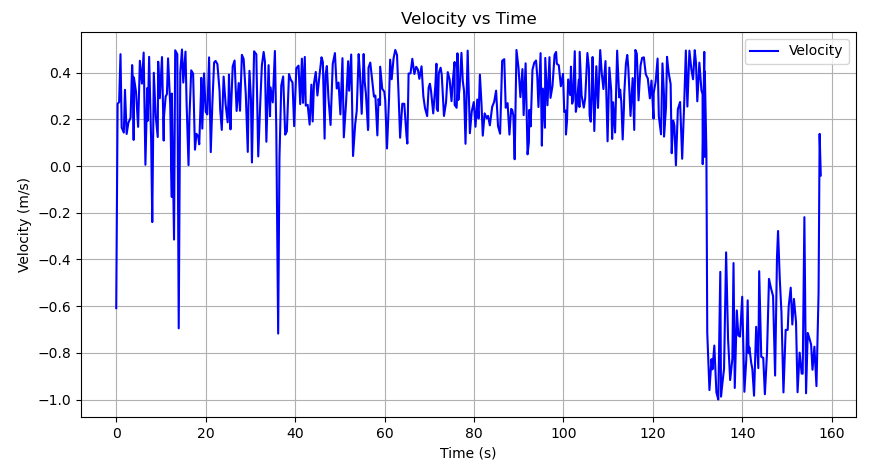
\includegraphics[width=0.7\textwidth]{2bVelocity.png} 
    \caption{Velocity vs time}
    \label{fig:2bVelocity}
\end{figure}

\begin{figure}[H]
    \centering
    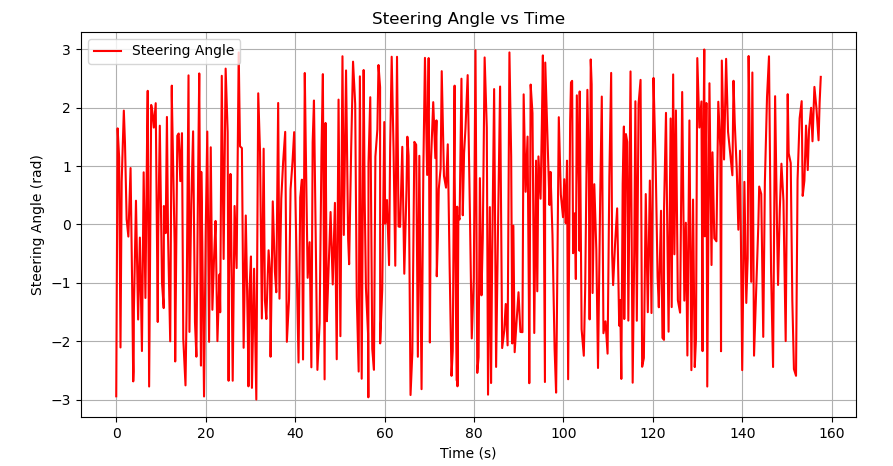
\includegraphics[width=0.7\textwidth]{2bSteeringAngle.png} 
    \caption{Steering Angle vs time}
    \label{fig:2bSteeringAngle}
\end{figure}

\subsection*{(c) Benchmark your implementation using three categories: number of valid solutions, path length, and computation time. Benchmark with 100 runs for \( |u_{\text{samples}}| \in \{1, 5, 10, 15\} \) and comment on the results.}
    
\subsection*{(d) Further restrict the steering angle limits to \( \phi \in \left[-\frac{\pi}{4}, \frac{\pi}{4}\right] \) and run benchmarks with \( |u_{\text{samples}}| = 5 \). Compare the previous results and discuss the differences, including possible causes.}

\subsection*{(e) Would a purely kinematic model (i.e., \( q = (x, y, \theta) \)) yield a feasible solution? Why or why not?}

A purely kinematic model with \( q = (x, y, \theta) \) would likely not yield a feasible solution for this parking problem. In the case of a car-like robot, a kinematic model does not account for the limitations in velocity and steering angle rate, which are essential for realistic motion in constrained environments. Without these constraints, the generated trajectory might include sharp turns or unrealistic accelerations that the car cannot physically perform, especially given the need for gradual adjustments when performing maneuvers such as parallel parking.

\subsection*{(f) (Optional) Use the state trajectory from your planner to render a video animation of the robot parking.}


\end{document}
